\subsection{Ristoratore} % --------------------- SECTION DEL RISTORATORE ---------------------%

    \subsubsection{Home Page}
    Una volta effettuato l'accesso come ristoratore, verrai reindirizzato alla tua Home Page personale. Composta da un calendario in cui è possibile selezionare il giorno desiderato per visualizzare le prenotazioni effettuate per quel giorno. Inoltre il calendario presenta per ciascun giorno delle possibili colorazioni diverse:
        \begin{itemize}
            \item Nessun colore: indica che non ci sono prenotazioni per quel giorno.
            \item Rosso: indica che ci sono prenotazioni in attesa di conferma per quel giorno.
            \item Verde: indica che ci sono prenotazioni confermate per quel giorno.
        \end{itemize}
        
        \begin{figure}[htbp]
            \centering
            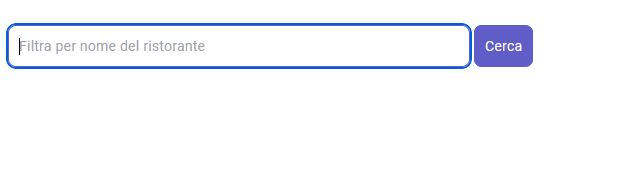
\includegraphics[width=0.5625\textwidth]{./img/Dettaglio.jpg}
            \caption{Calendario delle prenotazioni}
        \end{figure}
        
        A destra del calendario vengono visualizzate le prenotazioni effettuate del giorno selezionato, con la possibilità di visualizzare in dettaglio una prenotazione, semplicemente cliccando su di essa. Inoltre è possibile filtrarle per stato della prenotazione, orario o numero. Nella parte più a destra si hanno la lista di tutti gli ingredienti necessari a soddisfare la lista di prenotazioni visualizzata.
        
        \begin{figure}[htbp]
            \centering
            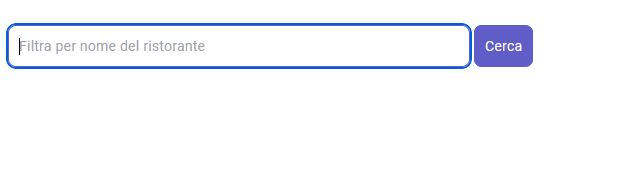
\includegraphics[width=0.5625\textwidth]{./img/Dettaglio.jpg}
            \caption{Barra di filtraggio delle prenotazioni}
        \end{figure}
        
        \begin{figure}[htbp]
            \centering
            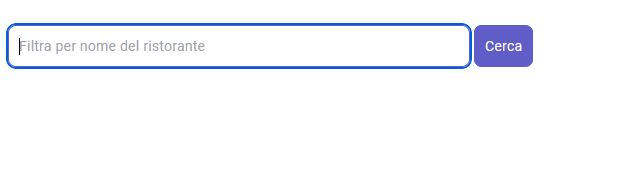
\includegraphics[width=0.5625\textwidth]{./img/Dettaglio.jpg}
            \caption{Lista degli ingredienti necessari per la giornata selezionata}
        \end{figure}

    \subsubsection{Barra di navigazione}
    La barra di navigazione in alto ti permette di accedere alle sezioni di esplorazione dei ristoranti, alla gestione delle prenotazioni, alla visualizzazione delle notifiche e al logout. Le funzionalità della barra di navigazione del ristoratore sono state precedentemente discusse nella sezione del cliente e quindi non verranno ripetute. Inoltre, la barra di navigazione del ristoratore include due funzionalità aggiuntive: "Piatti" e "Ingredienti".
        
        \begin{figure}[htbp]
            \centering
            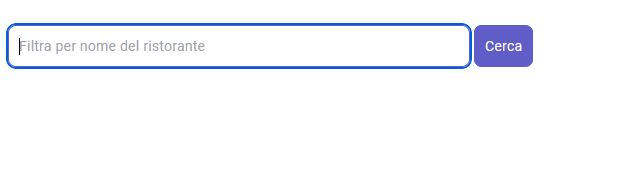
\includegraphics[width=0.5625\textwidth]{./img/Dettaglio.jpg}
            \caption{Barra di navigazione per il ristoratore}
        \end{figure}

    \subsubsection{Ingredienti}
    Questa sezione offre un'interfaccia intuitiva per la gestione degli ingredienti. Puoi inserire il nome del piatto e scegliere l'unità di misura tra le opzioni disponibili: g, ml, p, q.b. (grammi, millilitri, pezzi, quanto basta). Dopo aver inserito il nome e l'unità di misura, puoi salvare l'ingrediente al piatto. Sotto il modulo di inserimento, sono elencati tutti gli ingredienti presenti nel menu del ristorante. Puoi modificarli selezionando l'ingrediente (riconoscibile per lo sfondo celeste) e modificando i valori nel modulo, o eliminarli facendo clic sul pulsante "Elimina" a destra.
    
        \begin{figure}[htbp]
            \centering
            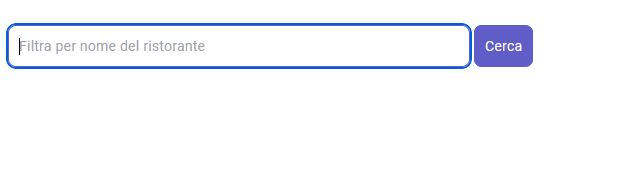
\includegraphics[width=0.5625\textwidth]{./img/Dettaglio.jpg}
            \caption{Modulo di gestione degli ingredienti}
        \end{figure}

    \subsubsection{Piatti}
    La sezione "Piatti" consente di creare e visualizzare tutti i piatti presenti nel menu del ristorante. Puoi creare un nuovo piatto utilizzando una scheda dedicata. Dopo aver cliccato sulla scheda, comparirà un modulo in cui inserire il nome del piatto, la descrizione, il prezzo e la foto del piatto.
    
        \begin{figure}[htbp]
            \centering
            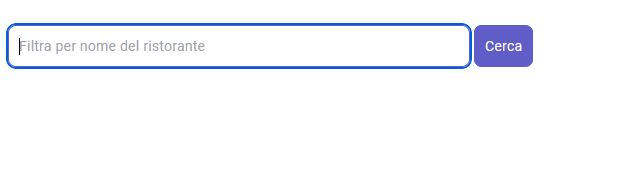
\includegraphics[width=0.5625\textwidth]{./img/Dettaglio.jpg}
            \caption{Card creazione piatto}
        \end{figure}

    \subsubsection{Aggiunta Ingredienti a un Piatto}
    Nell'elenco di tutti i piatti presenti nel menu del ristorante, è possibile visualizzare in dettaglio un piatto, semplicemente cliccando su di esso. Una volta in dettaglio, è possibile aggiungere un ingrediente per volta al piatto cliccando sul pulsante apposito in basso alla card del piatto. Si noti che per associare un ingrediente al piatto, l'ingrediente deve già esistere.
    
        \begin{figure}[htbp]
            \centering
            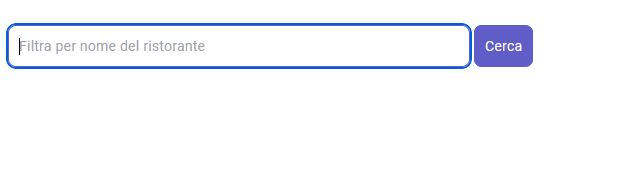
\includegraphics[width=0.5625\textwidth]{./img/Dettaglio.jpg}
            \caption{Pulsante aggiunta ingrediente ad un piatto}
        \end{figure}
        
    Inoltre, se si esegue un ulteriore click sulla card del piatto è possibile ritornare nel form, modificare i campi e salvare le modifiche, o addirittura eliminare il piatto.
    
        \begin{figure}[htbp]
            \centering
            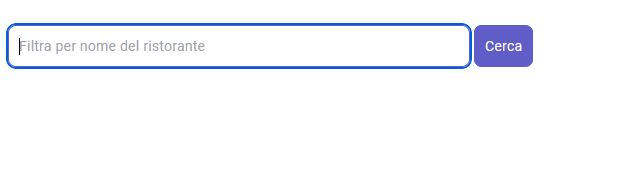
\includegraphics[width=0.5625\textwidth]{./img/Dettaglio.jpg}
            \caption{Modulo di modifica e eliminazione di un piatto}
        \end{figure}

    \subsubsection{Gestione prenotazioni}
    Tornando alla barra di navigazione, cliccando su "Prenotazioni" si accede alla pagina di gestione delle prenotazioni. Non è altro che lo stesso meccanismo che è presente nella home page del ristoratore solamente che non è presente il calendario.
